\documentclass{article}

\date{5 Mai 2024}
\usepackage[nb-sem=27, auteurs={Vangilluwen Hugo}]{../kholles}

\begin{document}
	\maketitle
	
	\begin{question_kholle}
		[{Soit $f \in \ContM{[a;b]}{}$. \\
		L'ensemble $\{ |f(t)| \;|\; t \in [a;b] \}$ admet une borne supérieur notée $\norminf{f}$.}]
		{Norme uniforme d'une fonction continue par morceaux}
		
		Montrons que sur chaque morceau, $f$ est bornée.
		
		Soit $\sigma = (x_i)_{0 \leqslant i \leqslant N} \in \mathcal{S}([a;b])$ adaptée à $f$.
		Soit $i \in \lient 0; N-1 \rient$. Posons $f_i = f_{|]x_i;x_{i+1}[}$.
		$f$ étant continue par morceaux, $\exists (l_i^+, l_{i-1}^-) \in \R^2 : \textlim{x}{x_i^+} f_i(x) = l_i^+ \wedge \textlim{x}{x_{i+1}^-} f_i(x) = l_{i+1}^-$.
		Nous pouvons donc prolonger $f_i$ en $\tilde{f_i}$ par continuité en $x_i$ et en $x_{i+1}$.
		Comme $f \in \Cont{0}{[a;b]}{}$, le théorème de Weierstrass s'applique : $\Im \tilde{f_i}$ est bornée (donc $f_i$ aussi). Ainsi $\norminf{f_i}$ est bien défini.
		
		\noindent $\{ |f(t)| \;|\; t \in [a;b] \}$ est : \begin{itemize}
			\item une partie de \R
			\item non vide car contenant $|f(x)|$.
			\item majorée par $\max \left( \{\norminf{f_i} | i \in \lient 0; N-1 \rient\} \cup \{\norminf{f_i} | i \in \lient 0; N-1 \rient\} \right)$ (ensemble admettant bien un plus grand élément puisque fini)
		\end{itemize}
		Donc $\norminf{f}$ est bien définie.
		\begin{figure}[H]
			\centering
			\begin{tikzpicture}
				\draw[->] (-0.5, 0) -- (5, 0);
				\draw[->] (0, -0.5) -- (0, 5);
				\draw (4, -0.1) node[anchor=north] {$1$} -- (4, 0.1);
				\draw (2, -0.1) node[anchor=north] {$\nicefrac{1}{2}$} -- (2, 0.1);
				\draw (-0.1, 4) node[anchor=east] {$1$} -- (0.1, 4);
				
				\draw[red] (0, 0) -- (2, 4) -- (4, 0);
				\filldraw[white, draw=red, densely dotted] (2, 3.95) circle (3pt);
				\filldraw[red] (2, 0) circle (2pt);
			\end{tikzpicture}
			\caption{$\norminf{f}$ peut ne pas être atteinte}
		\end{figure}
	\end{question_kholle}
	
	\begin{question_kholle}
		[Soit {$f \in \Cont{0}{[a;b]}{}$}.
		\begin{propositions}
			\item $\forall \varepsilon \in \R_+^*, \
			\exists \chi \in \mathcal{E}({[a;b]}, \R) :
			\norminf{f - \chi} \leqslant \varepsilon$
			\item $\forall \varepsilon \in \R_+^*, \
			\exists (\varphi, \psi) \in \mathcal{E}({[a;b]}, \R)^2 :
			\left\{ \begin{matrix}
				\varphi \leqslant f \leqslant \psi \\
				\norminf{\psi - \varphi} \leqslant \varepsilon
			\end{matrix} \right.$
		\end{propositions}]
		{Lemme d'approximation uniforme d'un fonction continue sur un segment par une fonction en escalier}
		
		Soit $f \in \Cont{0}{[a;b]}{}$. Soit $\varepsilon \in \R_+^*$ \fq. \\
		$(i)$ D'après le théorème de Heine, $f \in \ContU{[a;b]}{}$. Écrivons la définition de uniformément continue pour $\varepsilon$ :
		\begin{equation*}
			\exists \eta \in \R_ +^* : \ \forall (x, y) \in [a;b]^2, \
			|x - y| \leqslant \eta \implies |f(x) - f(y)| \leqslant \varepsilon
		\end{equation*}
		
		\begin{figure}[H]
			\centering
			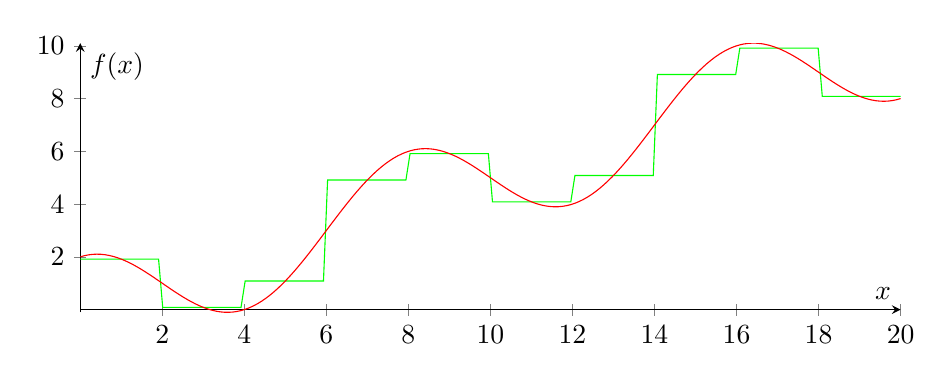
\begin{tikzpicture}
				\begin{axis}[
					axis lines = center,
					xlabel = $x$,
					ylabel = {$f(x)$},
					width=12cm,
					height=5cm
					]
					\addplot[
					domain=0:20,
					samples=200,
					color=green,
					]
					{2*cos((floor(x/2)*2+1)*45) + floor(x/2)+(1/2)};
					\addplot[
					domain=0:20,
					samples=200,
					color=red,
					]
					{2*cos(x*45) + x/2};
				\end{axis}
			\end{tikzpicture}
			\caption{Fonction en escalier "approximant" une fonction continue}
		\end{figure}
		
		\noindent Cherchons $N$ \tq $\frac{b - a}{N} \leqslant 2 \eta$. C'est-à-dire $N \geqslant \frac{b - a}{2 \eta}$.
		Posons donc $N = \lceil \frac{b - a}{2 \eta} \rceil$ et $\eta' = \frac{b-a}{N}$ de sorte que $\eta' \leqslant 2\eta$.
		
		Définissons $\chi \in \mathcal{E}({[a;b]}, \R)$ par
		\begin{equation*}
			\left| \begin{matrix}
				[a;b] &\rightarrow& \R \\
				x &\mapsto& \left\{ \begin{matrix}
					f(x) &\text{ si } \exists n \in \N : \ x = a + n \eta' \\
					f\left(a + \eta' \left( \lfloor \frac{x-a}{\eta'} \rfloor + \nicefrac{1}{2} \right) \right) &\text{ sinon }
				\end{matrix} \right.
			\end{matrix} \right.
		\end{equation*}
		Ceci est bien une fonction en escalier car $(a + k \eta')_{0 \leqslant k \leqslant N}$ est une subdivision adaptée. En effet, $\forall k \in \lient 0; N-1 \rient, \ f_{|]a+k\eta';a+(k+1)\eta'[} =f\left( a + \eta' \left( \lfloor \frac{x-a}{\eta'} \rfloor + \nicefrac{1}{2} \right) \right) \cdot \widetilde{1}_{]a+k\eta';a=(k+1)\eta'[}$.
		
		Soit $x \in [a; b]$.
		Si $\exists n \in \N : \ x = a + n \eta'$ alors $|f(x) - \chi(x)| = 0$.
		Sinon $0 \leqslant \frac{x - a} {\eta'} - \lfloor \frac{x-a}{\eta'} \rfloor \leqslant 1$.
		D'où $0 \leqslant (x - a) - \eta' \lfloor \frac{x-a}{\eta'} \rfloor \leqslant \eta'$.
		Donc, en enlevant $\nicefrac{\eta'}{2}$, $- \frac{\eta'}{2} \leqslant a + \eta' \left( \lfloor \frac{x-a}{2 \eta} \rfloor + \nicefrac{1}{2} \right) \leqslant \frac{\eta'}{2}$.
		Par définition de $\eta'$, \ $- \eta \leqslant a + \eta' \left( \lfloor \frac{x-a}{2 \eta} \rfloor + \nicefrac{1}{2} \right) \leqslant \eta$.
		Par définition de $\eta$, on a $|f(x) - f\left(a + 2 \eta \left( \lfloor \frac{x-a}{2 \eta} \rfloor + \nicefrac{1}{2} \right) \right)| \leqslant \varepsilon$.
		
		Ainsi, nous avons bien $\norminf{f - \chi} \leqslant \varepsilon$.
		\bigbreak
		
		$(ii)$ Écrivons la définition de uniformément continue pour $\varepsilon$ :
		\begin{equation*}
			\exists \eta \in \R_ +^* : \ \forall (x, y) \in [a;b]^2, \
			|x - y| \leqslant \eta \implies |f(x) - f(y)| \leqslant \varepsilon
		\end{equation*}
		Définissons $\varphi \in \mathcal{E}({[a;b]}, \R)$ par
		\begin{equation*}
			\left| \begin{matrix}
				[a;b] &\rightarrow& \R \\
				x &\mapsto& \left\{ \begin{matrix}
					f(x) &\text{ si } \exists n \in \N : \ x = a + n \eta \\
					\inf f\left( \; ]a + \eta \lfloor \frac{x-a}{\eta'} \rfloor; a + \eta \left( \lfloor \frac{x-a}{\eta'} \rfloor + 1 \right) [ \; \right) &\text{ sinon }
				\end{matrix} \right.
			\end{matrix} \right.
		\end{equation*}
		Définissons $\psi \in \mathcal{E}({[a;b]}, \R)$ par
		\begin{equation*}
			\left| \begin{matrix}
				[a;b] &\rightarrow& \R \\
				x &\mapsto& \left\{ \begin{matrix}
					f(x) &\text{ si } \exists n \in \N : \ x = a + n \eta \\
					\sup f\left( \; ] a + \eta \lfloor \frac{x-a}{\eta'} \rfloor; a + \eta \left( \lfloor \frac{x-a}{\eta'} \rfloor + 1\right)[ \; \right) &\text{ sinon }
				\end{matrix} \right.
			\end{matrix} \right.
		\end{equation*}
		Ces deux fonctions sont bien définies car $f_{|] a + \eta \lfloor \frac{x-a}{\eta'} \rfloor; a + \eta \left( \lfloor \frac{x-a}{\eta'} \rfloor + 1\right)[}$ est continue donc, d'après le théorème de Weiertraß, son image admet une borne inférieure et une borne supérieure.
		Elle sont bien en escalier.
		
		Par définition des bornes inférieures et supérieures, nous avons $\varphi \leqslant f \leqslant \psi$.
		De plus, pour $x \in [a;b]$ \fq, $f_{|] a + \eta \lfloor \frac{x-a}{\eta'} \rfloor; a + \eta \left( \lfloor \frac{x-a}{\eta'} \rfloor + 1\right)[}$ se prolonge par continuité et, d'après le théorème de Weiertraß, atteint ses bornes. Notons $f_i$ et $f_s$ les antécédents respectifs des bornes.
		$(f_i, f_s) \in ] a + \eta \lfloor \frac{x-a}{\eta'} \rfloor; a + \eta \left( \lfloor \frac{x-a}{\eta'} \rfloor + 1\right)[ ^2$ donc $\left|f_i - f_s\right| \leqslant \eta$.
		D'où $\left| f(f_i) - f(f_s) \right| \leqslant \varepsilon$.
		
		Ainsi, nous avons bien $\norminf{\psi - \varphi} \leqslant \varepsilon$.
	\end{question_kholle}
\end{document}